\mychapter{4}{MultiVariate Analysis}
\label{sec:unchapitre}

Now that we get background and signal samples we can perform the MVA for classification.\\
For this work the TMVA framework from ROOT was used. Multiple MVA were tested (fig. \ref{mva_multiple}) with default configuration then the 2
bests were selected for the tuning of their parameters.\\

\begin{figure}[h!]
\centering
    \begin{subfigure}[h!]{0.4\textwidth}
    \centering
        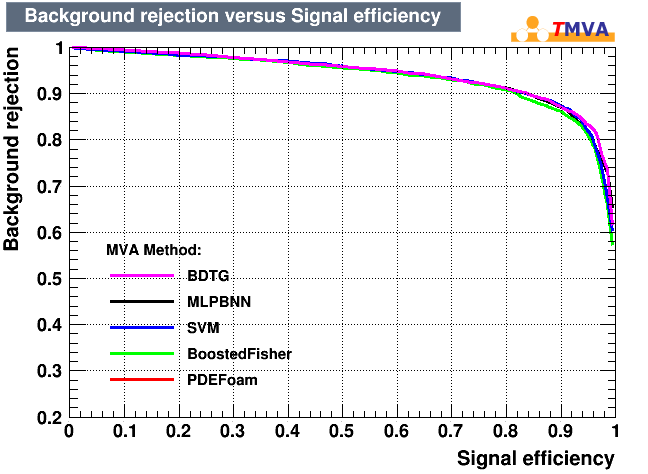
\includegraphics[width=\textwidth]{mva_multiple}
        \caption{ROC curve for the 5 bests MVA that has been tested.}
        \label{mva_multiple}
  \end{subfigure}
  ~
    \begin{subfigure}[h!]{0.4\textwidth}
    \centering
        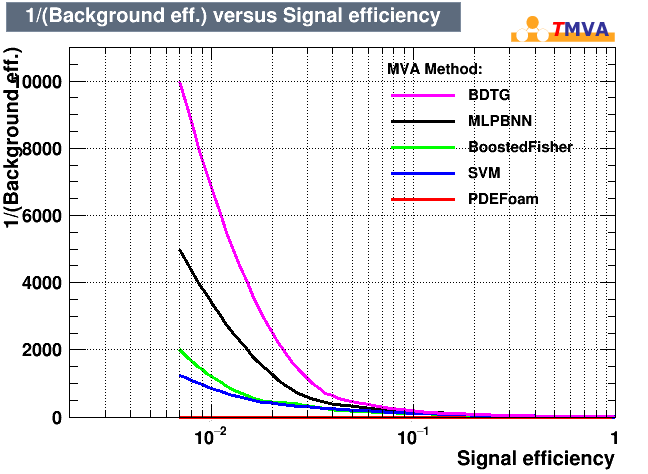
\includegraphics[width=\textwidth]{inv_mva_multiple.png}
        \caption{Inverse ROC curve for the 5 bests MVA that has been tested.}
        \label{inv_mva_multiple}
  \end{subfigure}
\end{figure}


\section{Artificial Neural Network}

An ANN is a multilayer perceptron with fully interconnected layers (fig. \ref{nn_arch}).
This ANN is used for classification, it is a function mapping an input vector $\vec{x_0}$ (input variables) to a scalar $y$ with $y \in [0;1]$ (classification category)\\
Here is the output of the ANN that has been trained for the next part of the analysis (fig. \ref{nn_output}).
\begin{figure}[h!]
\centering
    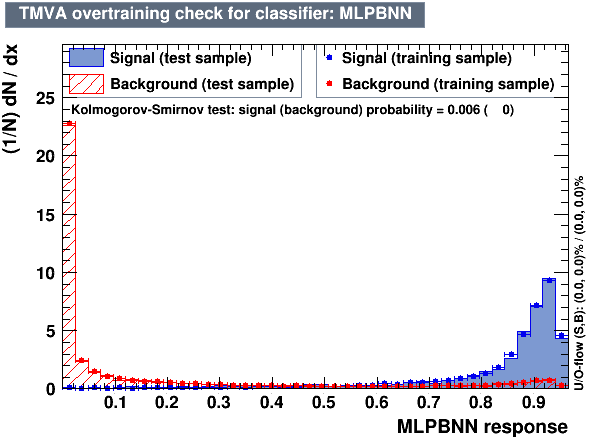
\includegraphics[width=0.6\textwidth]{nn_output}
    \caption{Artificial Neural Network response.}
    \label{nn_output}
\end{figure}


\subsection{Theory}

A neuron is referenced by his position in the network, a neuron $h_{i,j}(\vec{x_{j-1}}) \rightarrow h_{i,j}$ represent the i-th neuron of the j-th layer.\\
It sums all neuron's output in the (j-1)-th layer, weighted by their connection weight. This net sum is then evaluated through the activation function ( sigmoid, logistic, heaviside, linear, etc) (fig. \ref{one_neuron}).

\begin{figure}[h!]
\centering
    \begin{subfigure}[h!]{0.6\textwidth}
    \centering
    	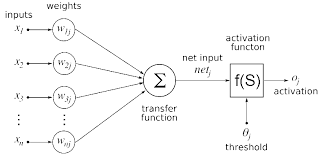
\includegraphics[width=\textwidth]{one_neuron}
    	\caption{Diagram of a single neuron algorithm.}
    	\label{one_neuron}
	\end{subfigure}
	~
    \begin{subfigure}[h!]{0.35\textwidth}
    \centering
    	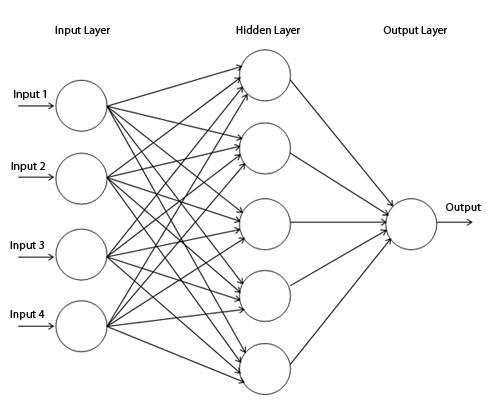
\includegraphics[width=\textwidth]{nn_arch}
    	\caption{Architecture of an artificial neural network with 4 input variables, one hidden layer, and one output neuron.}
    	\label{nn_arch}
	\end{subfigure}
\end{figure}


A lot of parameters are available for tuning :
\begin{description}
    \item [Input variable] Choice of input variable set, number of variables, choice of a Pre-processing method, etc.
    \item [ANN architecture] number of hidden layers, number of neurons per layer, choice of an activation function, etc.
    \item [Learning algorithm parameter] Choice of a learning method, choice of a regulator, value of learning rate, step size, weight decay rate, etc.
\end{description}

All of these cannot be optimize at the same time, so a choice has to be made.\\
The first parameter to be tune is the input variable set, a compromise has to be made in order to have the smallest input set but containing the most relevant information for classification.

\subsection{Input set optimization}

For this part an iterative process of optimization will be performed :
\begin{description}
	\item [step 1] Train MVA with full input variable set
	\item [step 2] Train N MVA removing one variable at a time
	\begin{description}
		\item [step 2.1] The MVA that succeed the best despite of having removed one variable, tells us that this variable wasn't revelant.
		\item [step 2.2] Remove this variable permanently, reiterate step 2 until no variable is left.
	\end{description}
	\item [final step] keep the input variable set of the best MVA
\end{description}

For evaluating the ANN multiple estimators has been tested :
\begin{description}
	\item [Mean Square Estimator (MSE)] $ MSE(\hat{\theta}) = E_{\hat{\theta}} [(\hat{\theta} - \theta)^2] =
    Var_{\hat{\theta}} + Bias(\hat{\theta}, \theta)^2$
	\item [Cross-Entropy (CE)] $ H(T,q) = -\sum_{i=1}^{N}{\frac{1}{N} log_2 q(x_i)}$
	\item [Overlapping criteria] $ = \sum_{i=1}^{N}{signal*background}$
\end{description}

\begin{figure}[h!]
    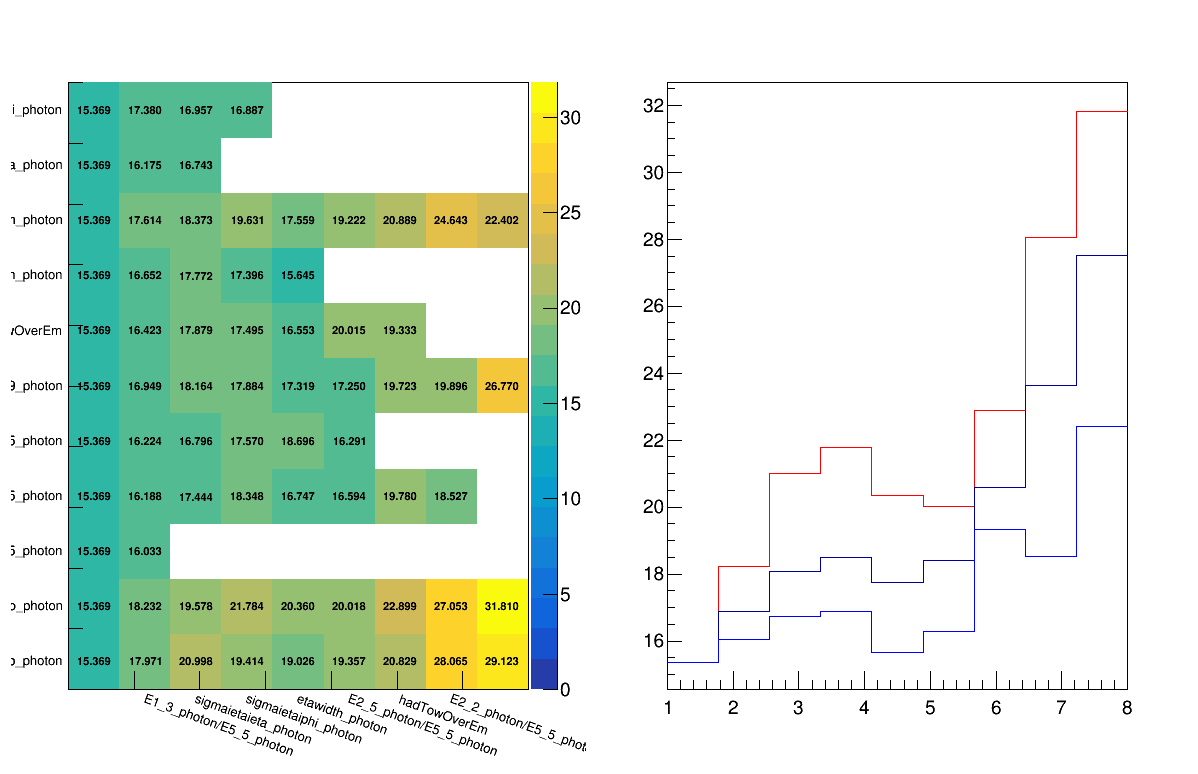
\includegraphics[width=\textwidth]{input_optim}
    \caption{Input variable set optimization.}
    \label{input_optim}
\end{figure}


\section{Boosted Decision Tree}

Being the best MVA method a BDT has been trained also for the next part of the analysis (fig. \ref{bdt_output}).
Multiple learning method has been used, the Gradient Boost Method was the most efficient one.
\begin{figure}[h!]
\centering
    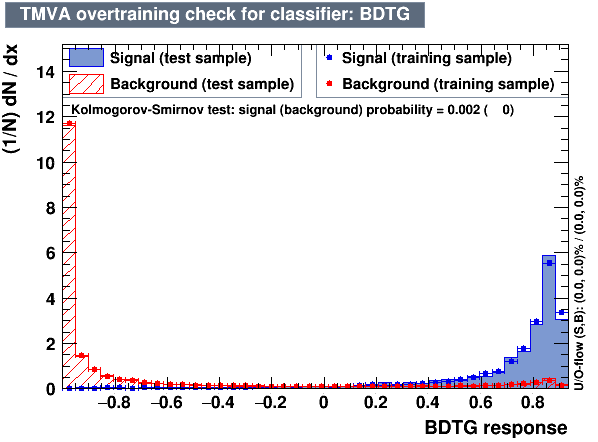
\includegraphics[width=0.6\textwidth]{bdt_output}
    \caption{Boosted Decision Tree response.}
    \label{bdt_output}
\end{figure}

\subsection{Theory}

BDT uses a decision tree in order to map from input variables to the event category (signal or background).
For this kind of classification tree, branches represent relations between variable or cuts on variables that lead to leaf representing category of the event.\\
The learning method was the "Gradient Boosting", the classification is done by combining together weak classifiers in an iteratively way.
A finir...

%%% Local Variables: 
%%% mode: latex
%%% TeX-master: "isae-report-template"
%%% End: 

